
\section{Metodología de análisis (UML-WAE)}
Como metodología de análisis utilizaré el estándar de facto UML.

\subsection{UML}
UML o Lenguaje de Modelado Unificado (Unified Modeling Language) fue creado para unificar las distintas técnicas que existían. Se trata de un lenguaje, principalmente, visual que nos permite visualizar, especificar, construir y documentar un sistema. Como lenguaje de modelado nos da las herramientas para especificar los métodos y/o procesos del sistema.

UML consta principalmente de dos puntos de vista. Un punto de vista estructural o estático en el cual se plasman estructuras estáticas compuesta por objetos, atributos, operaciones y relaciones. El otro punto de vista es dinámico o de comportamiento que permite establecer y/o especificar las colaboraciones entre las distintas partes del sistema. Este último punto de vista, además nos proporciona estados internos de nuestro sistema.

\subsubsection{Diagramas}
La metodología UML nos dota de un conjunto de diagramas para modelar.

\begin{figure}[htbp]
\centering
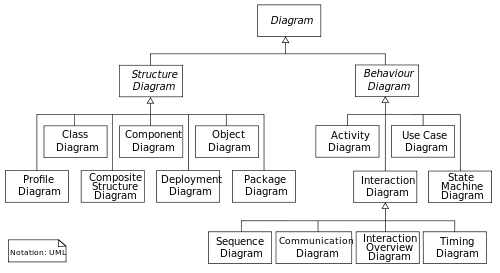
\includegraphics[width=\textwidth]{imagenes/diagramas}
\caption{Esquema de diagramas}
\label{fig:diagramas}
\end{figure}


El conjunto de diagramas se divide en dos grandes grupos:

\begin{itemize}
\item Diagramas de estructura. Se corresponde con el punto de vista estático. Entre los diagramas más destacados están:
\begin{itemize}
\item Diagrama de clases
\item Diagrama de componentes
\item Diagrama de paquete
\end{itemize}

\item Diagramas de comportamiento. Se corresponde con el punto de vista dinámico. Entre los más utilizados están:
\begin{itemize}
\item Diagrama de casos de usos
\item Diagrama de actividad
\item Diagrama de secuencia
\end{itemize}
\end{itemize}

UML 2 es extensible. Los mecanismo para personalizar y extender el UML son los perfiles y los estereotipos. UML-WAE utiliza los dos.

\subsubsection{UML-WAE}

Hoy en día, la mayoría de las aplicaciones se desarrollan entorno a la web, es decir, son aquellas aplicaciones que en su arquitectura y elementos principales están el navegador y el protocolo HTTP. Fue Jim Conallen, en 1988, quien definió una extensión del estándar UML para aplicaciones web. Esta extensión pasó a llamarse WAE (Web Application Extension) y se trata de la convención o extensión más aceptada por lo que podríamos a hablar de un estándar dentro de las distintas extensiones web de UML.

En un principio las aplicaciones web se basaban en un conjunto bien definidos de tecnologías. Con un servidor web, un cliente web capaz de comunicarse, vía protocolo HTTP, y de renderizar HTML. Con el tiempo se fueron sumando otras tecnologías como CSS, Javascripts, XML, Ajax, Comet, webGL, etc … Es fácil comprobar, que el desarrollo de una aplicación web, en principio sencilla se ha complicado con el paso del tiempo. De hecho, el propio HTML en principio sencillo y liviano se ha vuelto amplio y pesado. En el siguiente diagrama, podemos ver de forma esquemática un compendio del conjunto de tecnologías que se incorporan o que están en proceso de incorporación al HTML5.


Es evidente que tal conjunto de tecnologías y especificaciones llevan al desarrollador web a un sobre esfuerzo para estar al día. Pero también abre un sin fin de posibilidades que, ya hoy en día, podemos observar en la Internet.

WAE lo que nos ofrece, a los desarrolladores, es la posibilidad de modelar elementos como HTML, CSS, Javascripts, páginas de servidor, etc … Para ello, hizo uso de los mecanismos de extensión del UML:

\begin{itemize}
\item Estereotipo:  permite extender el vocabulario del UML, con el fin de crear nuevo elementos del modelo ya existente.  Se representa de la entre $\ll$ estereotipo$\gg$.
\begin{figure}[htbp]
\centering
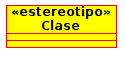
\includegraphics[width=0.2\textwidth]{imagenes/claseestereotipo}
\caption{Estereotipos}
\label{fig:claseestereotipo}
\end{figure}

\item Valores etiquetados: se trata de un conjunto de pares clave-valor que puede ir asociado a un elemento del modelo. Por ejemplo, {memoria=”4Gb”, núcleos=2}. En la versión 1.3, los “valores etiquetados” quedaron obsoletos A partir de UML2.0 se descartaron los “valores etiquetados”, en favor de los atributos. Por lo que, hoy en día se utilizan atributos para estos menesteres.
\begin{figure}[htbp]
\centering
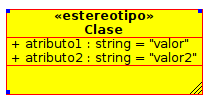
\includegraphics[width=0.3\textwidth]{imagenes/claseetiquetados}
\caption{Valores etiquetados}
\label{fig:claseetiquetados}
\end{figure}

\item Restricciones: se trata de una etiqueta. Su misión realizar asertos y/o especificar restricciones a una relación entre objetos del modelo. Por ejemplo, A {incluye} B.
\begin{figure}[htbp]
\centering
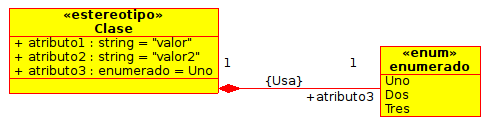
\includegraphics[width=0.7\textwidth]{imagenes/claserestricciones}
\caption{Estereotipos}
\label{fig:claseestereotipos}
\end{figure}

\end{itemize}

\subsubsection{Principales extensiones definidas por UML-WAE}

Las principales extensiones que podemos encontrar dentro de la extensión UML-WAE son:
\begin{itemize}
\item $\ll$ Server page $\gg$: representa una instancia de páginas de servidor. Estas páginas se caracterizan por tener scripts y/o código que se ejecutan en el servidor. (.php, .asp, .jsp).
\item $\ll$ Client page $\gg$: entidad que representa una una instancia de página que se renderiza en el cliente. Normalmente HTML y Javascripts.
\item $\ll$ Form $\gg$: representa a la entidad de formulario de un documento HTML. Se trata de una colección de campos de formularios HTML.
\item $\ll$ FrameSet $\gg$: representa el conjunto de marcos o frames que tiene una página.
\item $\ll$ Javascripts $\gg$: entidad que se refiere a una clase o entidad Javascripts.
\item $\ll$ Script Library $\gg$: componente de estereotipo Script Library representa una librería de funciones y/o rutinas que pueden ser incluidas en una página web.
\item $\ll$ Web Page $\gg$: componente de estereotipo Web page.
\item $\ll$ Submit $\gg$: una asociación de estereotipo submit son asociaciones de formularios HTML a otras páginas de clientes o servidor.
\item $\ll$ Build $\gg$: asociación utilizada para representar la salida de una página de servidor en una instancia de página de cliente.
\item $\ll$ Redirect $\gg$: sirve para especificar redirecciones realizada realizadas por cualquier página.
\item $\ll$ Link $\gg$: representa un ancho o enlace de una página de cliente a otra.
\end{itemize}
